\section{D\'eveloppement logiciel}

\subsection{Organisation}
\frame
{
\frametitle{Organisation du travail}


}

\subsection{Architecture}
\frame
{
\frametitle{Architecture de la solution propos\'ee}


\begin{minipage}{0.45\textwidth}
\begin{flushleft}
\begin{center}
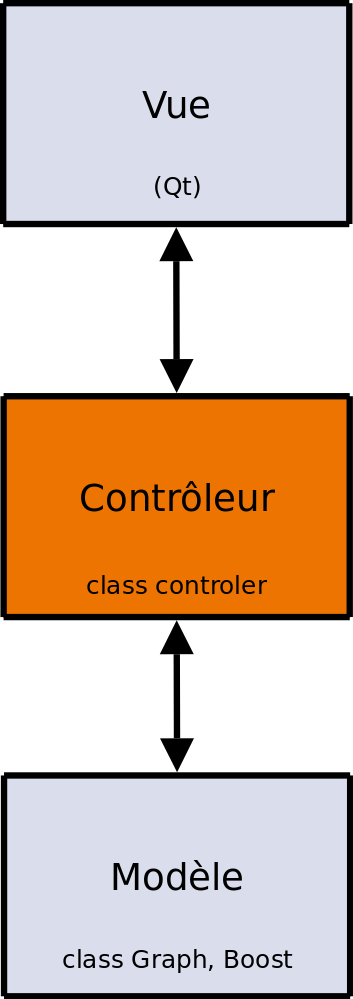
\includegraphics[height=0.95\textheight]{mvcScheme.png}
\end{center}
\end{flushleft}
\end{minipage}
\begin{minipage}{0.45\textwidth}
\begin{flushright}
\begin{block}{Vue}
\begin{center}
Interface graphique de l'utilisateur.
\end{center}
\end{block}
~\\
\begin{block}{Contrôleur}
\begin{center}
Gestion du dialogue entre la partie traitement et l'interface graphique.
\end{center}
\end{block}
~\\
\begin{block}{Modèle}
\begin{center}
Traitement et analyse des données.
\end{center}
\end{block}
\end{flushright}
\end{minipage}
}

\subsection{Boost}
\frame
{
\frametitle{D\'eveloppement avec la librairie Boost}


}